\begin{figure*}
    \centering
    \begin{subfigure}{0.68\linewidth}
      \fbox{\rule{0pt}{2in} \rule{.9\linewidth}{0pt}}
      \caption{An example of a subfigure.}
      \label{fig:short-a}
    \end{subfigure}
    \hfill
    \begin{subfigure}{0.28\linewidth}
      \fbox{\rule{0pt}{2in} \rule{.9\linewidth}{0pt}}
      \caption{Another example of a subfigure.}
      \label{fig:short-b}
    \end{subfigure}
    \caption{Example of a short caption, which should be centered.}
    \label{fig:short}
  \end{figure*}


  \begin{figure*}
    \centering
    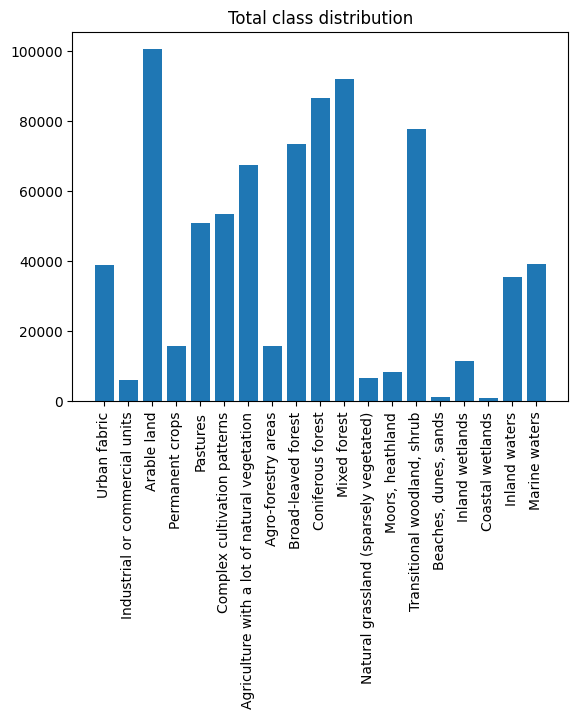
\includegraphics[width=\linewidth]{images/class_distribution.png}
    \caption{Example of a short caption, which should be centered.}
    \label{fig:short}
  \end{figure*}